
A better understanding of the counterfactual scenario that children would have faced if ABC/CARE were unavailable is useful in explaining the gender differences in the treatment effects. This requires us to identify the parameter in Equation~\eqref{eq:cont1}---the comparison between treatment and staying at home---and the parameter in Equation~\eqref{eq:cont2}---the analogous comparison to children who attended alternative preschools. These parameters are not identified by randomization into the treatment or control groups. The parents of the control-group children selected either to keep their children at home or take them to alternative preschools that were available when ABC/CARE was implemented. 

We rely on econometric methods for identification. In the main text, we rely on matching.\footnote{See \citet{Heckman_Ichimura_etal_1998_REStud} for a general discussion of the method, and an assessment of its practical implementation.} This method is practical in our case due to the small size of our samples. We show that the matching approach results in balanced samples (Table~\ref{tab:testing-matched-samples} in Appendix~\ref{app:matching-is-fun}). In Appendix~\ref{appendix:amethodology}, we show that instrumental-variable and control-function methods yield similar results but lack precision. In Appendix~\ref{appendix:results}, we discuss and document our choice of the matching variables, as well as other practical aspects of the implementation of this estimator.

Tables~\ref{table:massivealt} and~\ref{table:massivehome} provide analogous estimates to Table~\ref{table:massiveall}, using the different comparison groups (alternative preschool or stay at home). We argue that the $p$-values can be interpreted as magnitudes following \citet{Fisher_1935_Inference_JRSS}. In Table~\ref{table:massiveall}, with the full sample, the pattern of the $p$-values parallels that of the average effect sizes. In the comparison between the treatment group and those who attend alternative preschool, the  \citet{Rosenbaum_2005_Distribution_JRSS} $p$-value is significant for males more than for females. The exception to this is in education, in which the effect on females (0.332) is much larger than the effect of males (0.177). This pattern is reversed in the comparison between the treatment group and those who stayed at home. The exception to this is risky behavior, in which the effect on males (0.122) is much larger than the effect on females (0.054), even though the proportion of (significant) outcomes is the same. 

The intergenerational effect seen on the increase in parental income is strong across comparisons and genders. The effect size is larger in the comparison between treatment and those who stay at home, which is logical given that there are fewer labor market opportunities if the children stay at home. 

The effects on crime highlight that females were highly impacted by ABC/CARE, especially compared to those who attended alternative care. \citet{Garcia_Heckman_Leaf_etal_2017_Comp_CBA_Unpublished} find that even though the treatment effects on the crime outcomes are larger for women than for men, the men commit more socially expensive crimes. In the benefit/cost ratio that they compute, the effect of ABC/CARE on reducing individual male crimes is an important component. \citet{Garcia_etal_2019_ECE_IMHJ} discuss the crime results in more detail.

\begin{table}[!htpb]
\begin{threeparttable}
\caption{Combining Functions and Non-Parametric, Exact Tests, Treatment vs. Alternative} \label{table:massivealt}
\centering
 \begin{tabular}{l c c c c}
\toprule
 & Average & \% $ >0 $ & \% $ >0 $ , Significant & \citet{Rosenbaum_2005_Distribution_JRSS} \\
 & Effect Size & Treatment Effect & Treatment Effect & $ p $ -value \\
\midrule
\textbf{IQ} & & & & \\
\quad Females &  \textbf{    0.679} & \textbf{  100.000} & \textbf{  100.000} & .977 \\
\quad Males &  \textbf{    0.544} & \textbf{  100.000} & \textbf{  100.000} & .012 \\
\midrule
\textbf{Achievement} & & & & \\
\quad Females &  \textbf{    0.680} & \textbf{  100.000} & \textbf{  100.000} & .183 \\
\quad Males &  \textbf{    0.232} & \textbf{  100.000} & \textbf{   80.000} & .448 \\
\midrule
\textbf{Social-emotional} & & & & \\
\quad Females &  \textbf{    0.348} & \textbf{   85.714} & \textbf{   57.143} & .898 \\
\quad Males &  \textbf{    0.081} & \textbf{   64.286} & \textbf{   28.571} & .901 \\
\midrule
\textbf{Parental Income} & & & & \\
\quad Females &  \textbf{    0.211} & \textbf{  100.000} & \textbf{   60.000} & .052 \\
\quad Males &  \textbf{    0.299} & \textbf{  100.000} & \textbf{   60.000} & .061 \\
\midrule
\textbf{Parenting} & & & & \\
\quad Females &  \textbf{    0.173} & \textbf{  100.000} &    20.000 & .183 \\
\quad Males &     -0.003 & \textbf{   60.000} &     0.000 & .061 \\
\midrule
\textbf{Education} & & & & \\
\quad Females &  \textbf{    0.332} & \textbf{   83.333} & \textbf{   83.333} & .052 \\
\quad Males &  \textbf{    0.177} & \textbf{   83.333} & \textbf{   33.333} & .448 \\
\midrule
\textbf{Employment} & & & & \\
\quad Females &  \textbf{    0.164} & \textbf{  100.000} & \textbf{   50.000} & .429 \\
\quad Males &  \textbf{    0.491} & \textbf{  100.000} & \textbf{   50.000} & .448 \\
\midrule
\textbf{Crime} & & & & \\
\quad Females &  \textbf{    0.334} & \textbf{  100.000} & \textbf{  100.000} & .898 \\
\quad Males &     -0.322 & \textbf{   33.333} &     0.000 & .448 \\
\midrule
\textbf{Risky Behavior} & & & & \\
\quad Females &  \textbf{    0.140} & \textbf{  100.000} &     0.000 & .708 \\
\quad Males &     -0.050 & \textbf{   25.000} & \textbf{   25.000} & .448 \\
\midrule
\textbf{Health} & & & & \\
\quad Females &      0.093 & \textbf{   68.750} & \textbf{   31.250} & .835 \\
\quad Males &      0.080 & \textbf{   56.250} & \textbf{   31.250} & 0 \\
\bottomrule
\end{tabular}
% This file generated by: /scripts/abccare/genderdifferences/abccare-gdiff-raw-rosenbaum-table-big.do
 
\begin{tablenotes}
\footnotesize
\item \footnotesize \textbf{Note:} This table displays summaries of treatment effects by outcome category and gender. The comparison group is the control-group children who attend alternatives. The panels contains statistics calculated using outcomes grouped by category. The average effect size is calculated by averaging over the effect size of the outcomes in the outcome category. The effect sizes of the individual outcomes are calculated by dividing the coefficient by the standard deviation of the control group. We test these three statistics bootstrapped $p$-values. For the proportion of outcomes that are positive and significant, we do a ``double bootstrap'' procedure. The null hypothesis for the effect sizes is that they are 0. The null hypothesis for the proportion of outcomes that are (significantly) positive is that they are (10\%) 50\%. Bolded statistics are significant at the 10\% level. The \citet{Rosenbaum_2005_Distribution_JRSS} $p$-value originates from a test where the null is a common joint distribution of the variables in each category. Statistics significant at the $0.10$ level are bolded.
\end{tablenotes}
\end{threeparttable}
\end{table}

\begin{table}[!htpb]
\begin{threeparttable}
\caption{Combining Functions and Non-Parametric, Exact Tests, Treatment vs. Home Care} \label{table:massivehome}
\centering
 \begin{tabular}{l c c c c}
\toprule
 & Average & \% $ >0 $ & \% $ >0 $ , Significant & \citet{Rosenbaum_2005_Distribution_JRSS} \\
 & Effect Size & Treatment Effect & Treatment Effect & $ p $ -value \\
\midrule
\textbf{IQ} & & & & \\
\quad Females &  \textbf{    0.703} & \textbf{  100.000} & \textbf{  100.000} & .061 \\
\quad Males &  \textbf{    0.829} & \textbf{  100.000} & \textbf{  100.000} & .02 \\
\midrule
\textbf{Achievement} & & & & \\
\quad Females &  \textbf{    0.397} & \textbf{  100.000} & \textbf{   80.000} & .414 \\
\quad Males &  \textbf{    0.446} & \textbf{  100.000} & \textbf{   80.000} & .823 \\
\midrule
\textbf{Social-emotional} & & & & \\
\quad Females &  \textbf{    0.221} & \textbf{   71.429} & \textbf{   64.286} & .414 \\
\quad Males &  \textbf{    0.237} & \textbf{   92.857} & \textbf{   64.286} & .394 \\
\midrule
\textbf{Parental Income} & & & & \\
\quad Females &  \textbf{    0.336} & \textbf{  100.000} & \textbf{   80.000} & .061 \\
\quad Males &  \textbf{    0.460} & \textbf{  100.000} & \textbf{  100.000} & .053 \\
\midrule
\textbf{Parenting} & & & & \\
\quad Females &  \textbf{    0.255} & \textbf{  100.000} & \textbf{   80.000} & .414 \\
\quad Males &  \textbf{    0.290} & \textbf{  100.000} & \textbf{   80.000} & .823 \\
\midrule
\textbf{Education} & & & & \\
\quad Females &  \textbf{    0.292} & \textbf{   83.333} & \textbf{   50.000} & .061 \\
\quad Males &  \textbf{    0.311} & \textbf{   83.333} & \textbf{   50.000} & .394 \\
\midrule
\textbf{Employment} & & & & \\
\quad Females &  \textbf{    0.424} & \textbf{  100.000} & \textbf{  100.000} & .867 \\
\quad Males &  \textbf{    0.389} & \textbf{  100.000} & \textbf{  100.000} & .394 \\
\midrule
\textbf{Crime} & & & & \\
\quad Females &     -0.278 & \textbf{   33.333} &     0.000 & .024 \\
\quad Males &      0.112 & \textbf{   66.667} & \textbf{   66.667} & .394 \\
\midrule
\textbf{Risky Behavior} & & & & \\
\quad Females &      0.054 & \textbf{   50.000} & \textbf{   25.000} & .414 \\
\quad Males &  \textbf{    0.122} & \textbf{   50.000} & \textbf{   25.000} & .002 \\
\midrule
\textbf{Health} & & & & \\
\quad Females &      0.005 & \textbf{   56.250} & \textbf{   25.000} & .002 \\
\quad Males &  \textbf{    0.075} & \textbf{   80.000} & \textbf{   46.667} & .02 \\
\bottomrule
\end{tabular}
% This file generated by: /scripts/abccare/genderdifferences/abccare-gdiff-raw-rosenbaum-table-big.do
 
\begin{tablenotes}
\footnotesize
\item  \footnotesize \textbf{Note:} This table displays summaries of treatment effects by outcome category and gender. The comparison group is the control-group children who stay at home.The panels contains statistics calculated using outcomes grouped by category. The average effect size is calculated by averaging over the effect size of the outcomes in the outcome category. The effect sizes of the individual outcomes are calculated by dividing the coefficient by the standard deviation of the control group. We test these three statistics bootstrapped $p$-values. For the proportion of outcomes that are positive and significant, we do a ``double bootstrap'' procedure. The null hypothesis for the effect sizes is that they are 0. The null hypothesis for the proportion of outcomes that are (significantly) positive is that they are (10\%) 50\%. Bolded statistics are significant at the 10\% level. The \citet{Rosenbaum_2005_Distribution_JRSS} $p$-value originates from a test where the null is a common joint distribution of the variables in each category. Statistics significant at the $0.10$ level are bolded.
\end{tablenotes}
\end{threeparttable}
\end{table}

\begin{sidewaysfigure}[!htpb]
\centering
\caption{Gender and Baseline Socioeconomic Disadvantage in the Control Group} \label{figure:socdis}
\begin{subfigure}[h]{0.4\textwidth}
	\centering
	\caption{Take-up of Alternatives by Gender} \label{figure:altgender}
	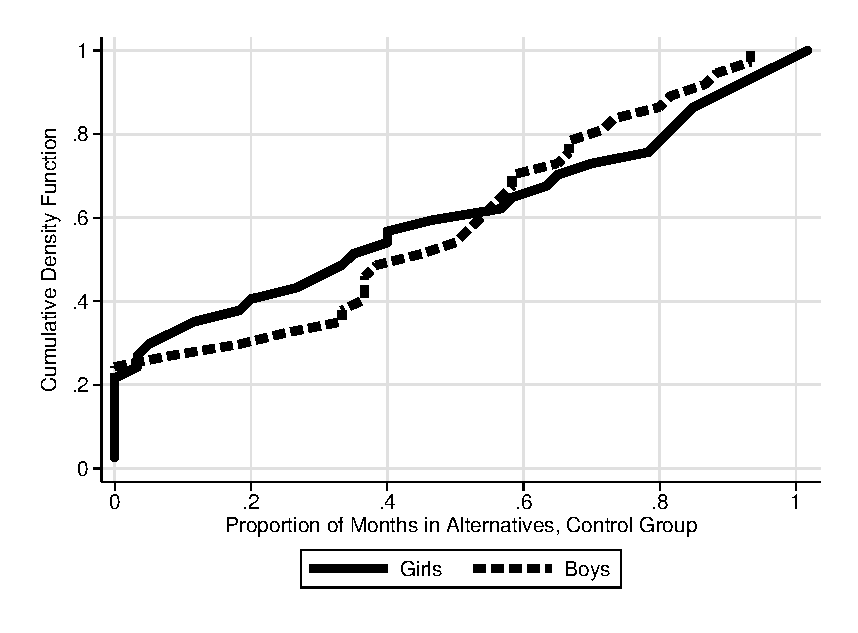
\includegraphics[width=\textwidth]{output/abccare_controlcontamination_boysgirls}
\end{subfigure}%
\begin{subfigure}[h]{0.4\textwidth}
	\centering
	\caption{Socioeconomic Disadvantage by Gender} \label{figure:disadgender}
	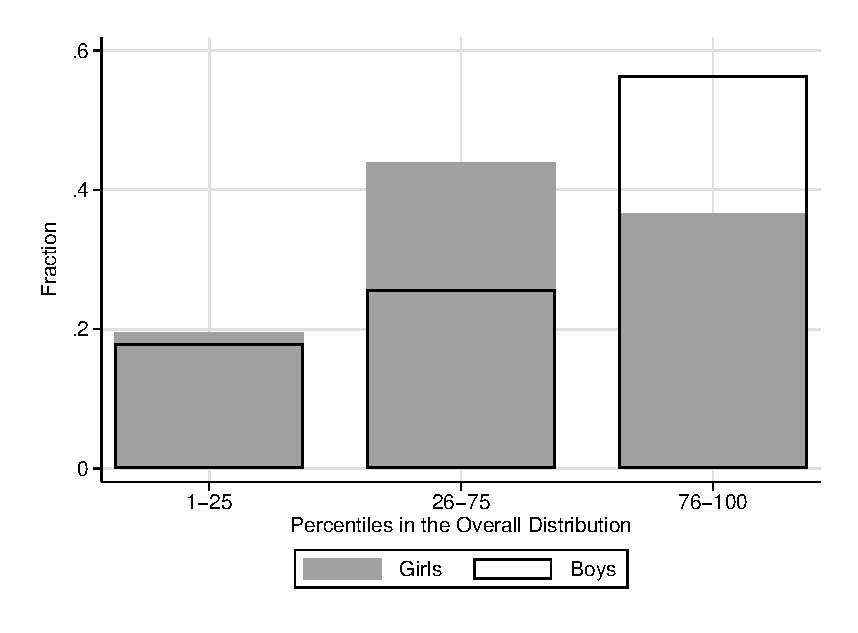
\includegraphics[width=\textwidth]{output/factorbase_girlsboyscompare}
\end{subfigure}
\begin{subfigure}[h]{0.4\textwidth}
	\centering
	\caption{Disadvantage by Take-up of Alternatives, Girls} \label{figure:disadgirls}
	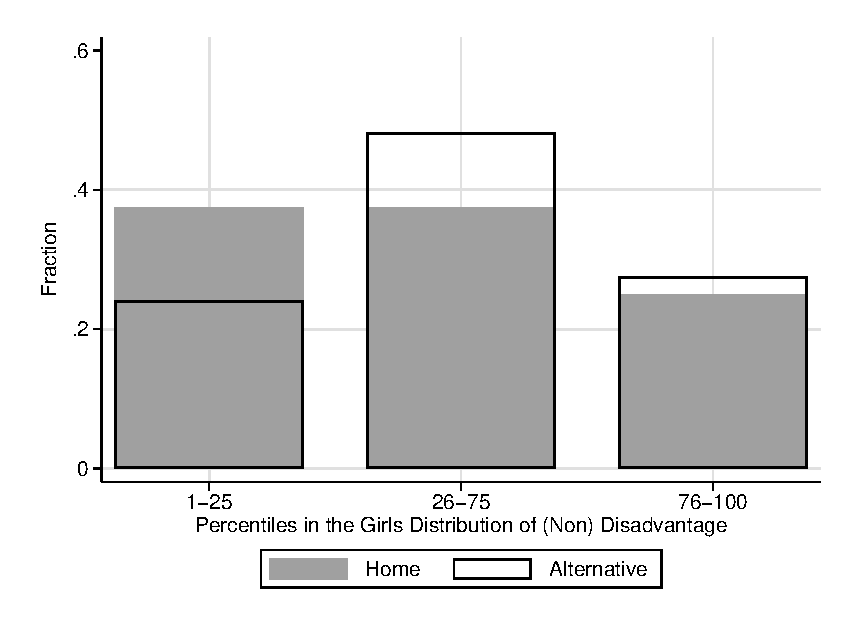
\includegraphics[width=\textwidth]{output/factorbase_wgirlscompare}
\end{subfigure}%
\begin{subfigure}[h]{0.4\textwidth}
	\centering
	\caption{Disadvantage by Take-up of Alternatives, Boys} \label{figure:disadboys}
	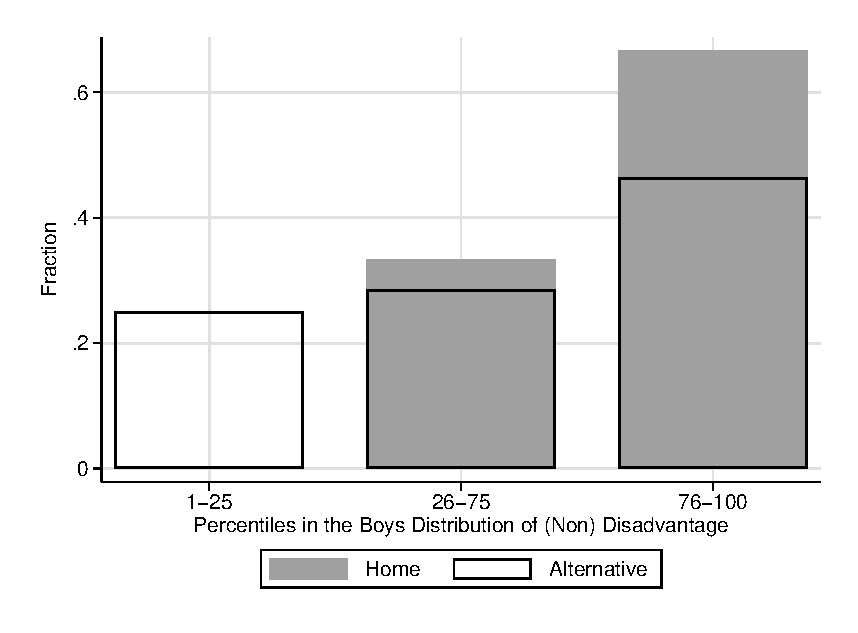
\includegraphics[width=\textwidth]{output/factorbase_wboyscompare}
\end{subfigure}
\footnotesize
\justify
\textbf{Note:} Panel (a) displays the cumulative distribution function of enrollment in alternatives by gender. Panel (b) displays how girls and boys separately fit into the overall (girls and boys pooled) distribution of socioeconomic disadvantage. Panel (c) displays how girls who did not enroll and girls who enrolled in alternatives fit into the overall female distribution of socioeconomic disadvantage. Panel (d) is analogous to Panel (c) for boys. Our measure of socioeconomic disadvantage is a latent of the following variables: Mother's age, education, IQ, marital status, and employment, as well as number of siblings and father's presence at home.
\end{sidewaysfigure}

The difference in the comparison of treatment to staying at home and alternative preschools suggests that boys and girls faced different situations of socio-economic disadvantaged at home. Figure~\ref{figure:socdis} investigates this. We start by noting that take-up of alternatives does not differ by gender (Panel~\ref{figure:altgender}). What does differ by gender is socioeconomic disadvantage. We create a latent measure of socioeconomic disadvantage at baseline using the following variables: Mother's age, education, IQ, marital status, and employment, as well as number of children and father's presence at home. We assess how girls and boys fit into the overall distribution of this latent in the control group. Boys are disproportionately more advantaged than girls (Panel~\ref{figure:disadgender}).\footnote{Note that this measure is based on baseline characteristics, so this result holds for the treatment group.} Because girls' families were more resource constrained if compared to their male counterparts, girls in the control group were taken care of in a more disadvantaged environment or went to lower-quality preschools. Thus, they benefited more than boys if compared to the next best alternative as perceived by their parents, as documented in Section~\ref{sec:treatment-effects}.


\begin{table}[!htpb]
\begin{threeparttable}
\caption{Gender and Baseline Socioeconomic Disadvantage in the Control Group, Tests} \label{table:disadtests}
\centering 
\begin{tabularx}{16.5cm}{XcX}
& \begin{tabular}{cccc}
\toprule
Males vs. Females & & \mc{2}{c}{Alt. vs. Home} \\
\cmidrule(lr){1-2} \cmidrule(lr){3-4}
Control Group & & Males & Females \\
\midrule
\textbf{0.007} & & \textbf{0.006} & 0.110 \\
\bottomrule
\end{tabular}

% Control, males vs. females: distance between: factor of m_age_base, m_ed_base, m_iq_base, hh_sibs_base, hrabc_index

% Alt. vs home: factor of m_age_base, m_ed_base, m_iq_base, hh_sibs_base, hrabc_index & 
\end{tabularx}
\begin{tablenotes}
\footnotesize
\item \textbf{Note:} This table presents the null of a common joint distribution of the variables composing our measure of socioeconomic disadvantage (mother's age, education, IQ, marital status, and employment, as well as number of siblings and father's presence at home) between males and females in the control group and between children who attended  alternative preschool and who stayed at home (within control-group boys or within control-group girls). The $p$-values follow \citet{Rosenbaum_2005_Distribution_JRSS}. Under the null hypothesis, the pairs with the closest distance in disadvantage would be comprised of one male and one female (for the comparison of males vs. females). Rejecting the null implies that the distributions are significantly different. Statistics significant at the $0.10$ level are bolded.
\end{tablenotes}
\end{threeparttable}
\end{table}

We formally test the difference in disadvantage across boys and girls in Table~\ref{table:disadtests}. We reject the null of a common joint distribution of the variables composing our measure of socioeconomic disadvantage across girls and boys (at baseline). In Panels~\ref{figure:disadgirls} and~\ref{figure:disadboys} of Figure~\ref{figure:socdis}, we further dissect socioeconomic disadvantage within genders, and provide the corresponding tests in Table~\ref{table:disadtests}. 


Parents of more advantaged girls are more likely to send their daughters to alternative preschools. Parents of more advantaged boys are more likely to send keep their sons at home. This provides an explanation why girls benefited more from treatment if compared to staying at home, which would be a more disadvantaged environment if compared to the male environments. Boys benefited more from treatment if compared to attending alternatives given that their parents plausibly sent them to lower-quality alternatives due to a lack of resources or the alternatives were worse complements to home learning environments. 











